%========================================================
\section{ORE Data Flow}\label{sec:process}
%========================================================

The core processing steps followed in ORE to produce risk analytics results are sketched in Figure \ref{fig_process}.
All ORE calculations and outputs are generated in three fundamental process steps as indicated in the three boxes in the
upper part of the figure. In each of these steps appropriate data (described below) is loaded and results are generated,
either in the form of a human readable report, or in an intermediate step as pure data files (e.g. NPV data, exposure data).
\begin{figure}[h]
\begin{center}
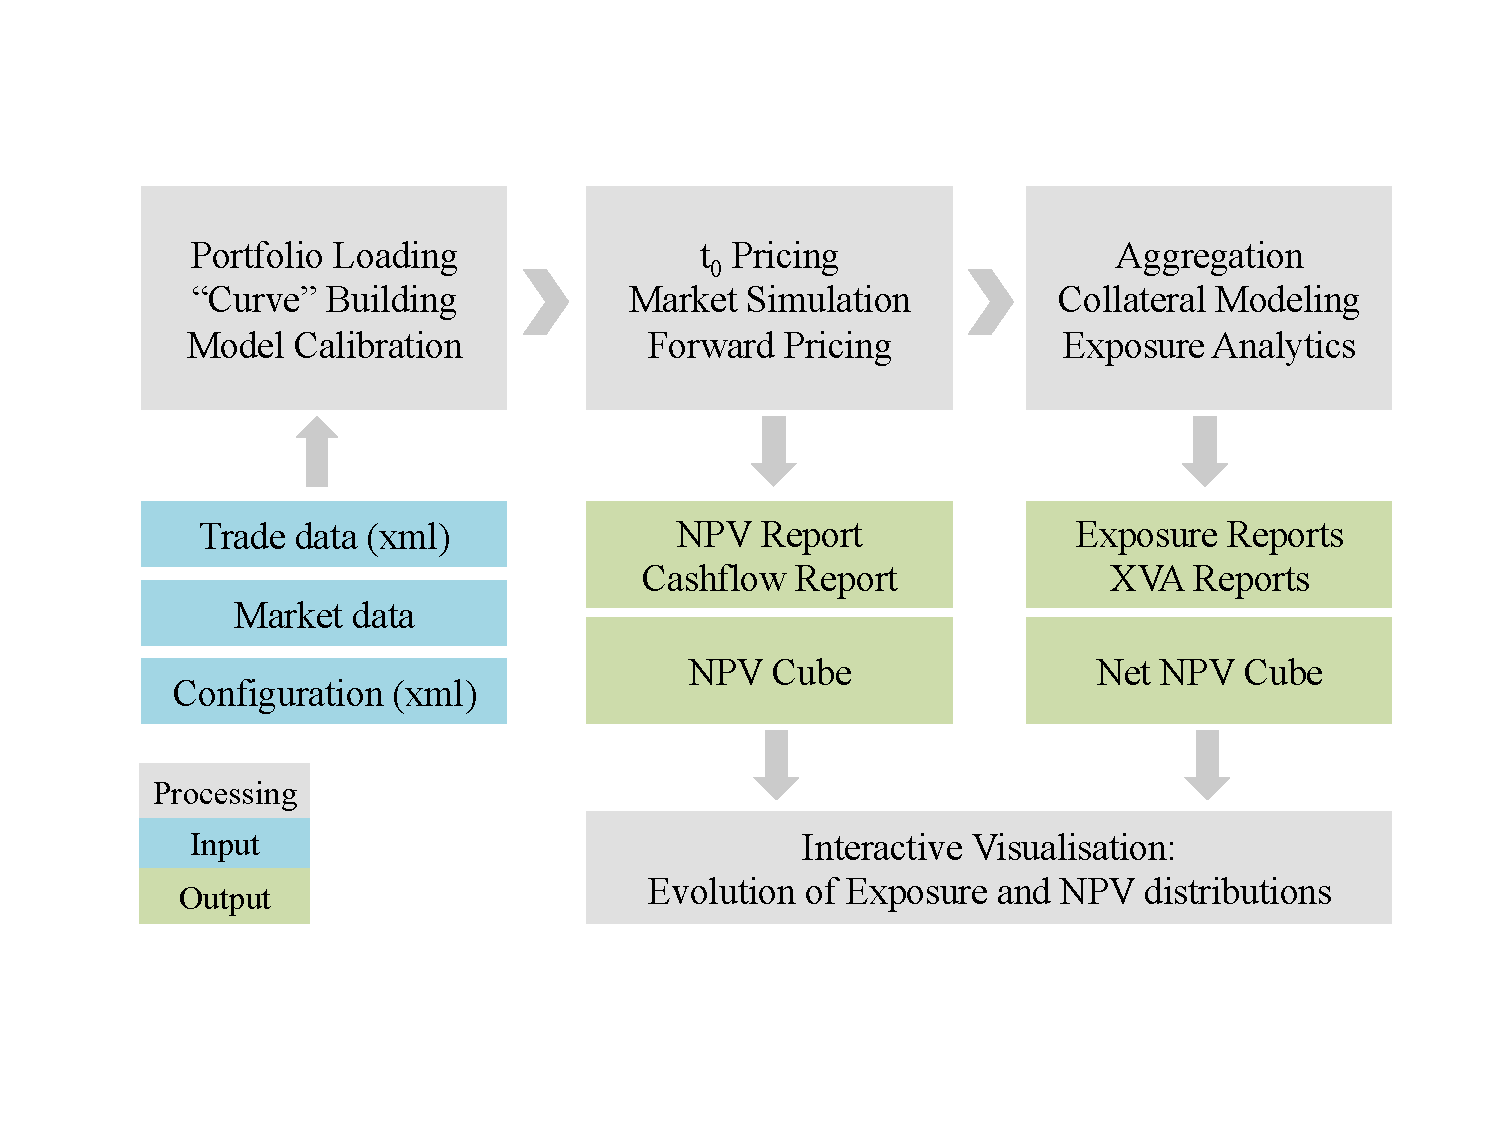
\includegraphics[scale=0.6]{process.pdf}
\end{center}
\caption{Sketch of the ORE process, inputs and outputs. }
\label{fig_process}
\end{figure}

The overall ORE process needs to be parametrised using a set of configuration XML files which is the subject of section
\ref{sec:configuration}. The portfolio is provided in XML format which is explained in detail in \cite{products} and \ref{sec:nettingsetinput}. Note that ORE comes with 'Schema' files for all supported
products so that any portfolio xml file can be validated before running through ORE. Market data is provided in a simple
three-column text file with unique human-readable labelling of market data points, as explained in section
\ref{sec:market_data}.  \\

The first processing step (upper left box) then comprises 
\begin{itemize}
\item loading the portfolio to be analysed, 
\item building any yield curves or other 'term structures' needed for pricing, 
\item calibration of pricing and simulation models.
\end{itemize}

The second processing step (upper middle box) is then 
\begin{itemize}
\item portfolio valuation, cash flow generation,
\item going forward - conventional risk analysis such as sensitivity analysis and stress testing, standard-rule capital
  calculations such as SA-CCR, etc,
\item and in particular, more time-consuming, the market simulation and portfolio valuation through time under Monte
  Carlo scenarios.
\end{itemize}
This process step produces several reports (NPV, cashflows etc) and in particular an {\bf NPV cube}, i.e. NPVs per
trade, scenario and future evaluation date. The cube is written to a file in both condensed binary and human-readable
text format.  \\

The third processing step (upper right box) performs more 'sophisticated' risk ana\-ly\-sis by post-processing the NPV
cube data:
\begin{itemize}
\item aggregating over trades per netting set, 
\item applying collateral rules to compute simulated variation margin as well as simulated (dynamic) initial margin
  posting,
\item computing various XVAs including CVA, DVA, FVA, MVA for all netting sets, with and without taking collateral
  (variation and initial margin) into account, on demand with allocation to the trade level.
\end{itemize}
The outputs of this process step are XVA reports and the 'net' NPV cube, i.e. after aggregation, netting and collateral. \\

The example section \ref{sec:examples} demonstrates for representative product types how the described processing steps
can be combined in a simple batch process which produces the mentioned reports, output files and exposure evolution
graphs in one 'go'.

%Moreover, both NPV cubes can be further analysed interactively using a visualisation tool introduced in section
%\ref{sec:jupyter}. And finally, sections \ref{sec:calc} and \ref{sec:excel} demonstrate how ORE processes can be
%launched in spreadsheets and key results presented automatically within the same sheet.
